\apendice{Documentación técnica de programación}

\section{Introducción}

En esta sección encontrarás información detallada sobre la estructura del código. Esta documentación está diseñada para brindar claridad y orientación a los desarrolladores, facilitando el mantenimiento, la expansión y la comprensión del código fuente del proyecto.

\section{Estructura de directorios}
Cada parte del proyecto está contenido en una carpeta.

\begin{table}[htbp]
\begin{center}
\caption{Directorios que contienen partes del proyecto.}
\begin{tabular}{|l|l|} %|c|c|
\hline
\rowcolor[HTML]{C0C0C0} 
\textbf{Carpeta} & \textbf{Descripción}\\ \hline
Hardware &  Implementación del harware\\ \hline
nodeMqtt & Servicio para almacenar datos en una base de datos \\ \hline
InverIoT &  Aplicación de escritorio\\ \hline
dashboard &  Dashboard web accesible desde internet \\ \hline
AnalisisDatos & Limpieza de datos y resumen estadístico \\ \hline
TFG & Documentación del proyecto \\ \hline
\end{tabular}
\end{center}
\end{table}

\subsection{Hardware}
Contiene detalles de las conexiones y código de programación en Micropython~\cite{wiki:micropython}.

El directorio \textbf{fritzing}~\ref{tabla:fritzing} contiene los esquemas de conexiones entre la Raspberry Pi Pico W, los módulos, sensores y leds RGB.

El directorio \textbf{micropython}~\ref{tabla:micropython} contiene el código de programación para controlar el hardware.

Respecto al directorio \textbf{lib}~\ref{tabla:lib} los archivos que empiezan con "mi\_" son implementaciones mías que hizo posible reducir la cantidad de líneas de código de programación en el archivo \textbf{main.py}.

\begin{figure}[h]
\centering
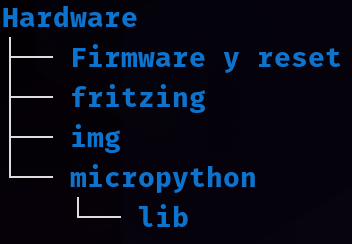
\includegraphics[width=0.9\textwidth]{img/diagramas/directorios_hardware.png}
\caption{Rama de directorios de hardware.}
\end{figure}

\begin{table}[htbp]
\begin{center}
\caption{Directorio: Firmware y reset.}
\begin{tabular}{|l|l|} %|c|c|
\hline
\rowcolor[HTML]{C0C0C0} 
\textbf{Nombre de Archivo} & \textbf{Descripción}\\ \hline
flash\_nuke.uf2 & Firmware para configuración de fábrica\\ \hline
RPI\_PICO\_W-20240105-v1.22.1.uf2 & Firmware oficial de la RPI PICO W\\ \hline
\end{tabular}
\end{center}
\end{table}

\begin{table}[htbp]
\begin{center}
	\caption{Directorio: Fritzing.}
\begin{tabular}{|l|} %|c|c|
\hline
\rowcolor[HTML]{C0C0C0} 
\textbf{Nombre de Archivo}\\ \hline
BH1750.fzz  \\ \hline
conexiones.fzz  \\ \hline
DHT22\_humedad\_temperatura.fzz  \\ \hline
leds\_rgb.fzz  \\ \hline
oled\_i2c\_168x64.fzz  \\ \hline
Sensor\_humedad\_suelo.fzz \\ \hline
\end{tabular}
\label{tabla:fritzing}
\end{center}
\end{table}

\begin{table}[htbp]
\begin{center}
\caption{Directorio: micropython.}
\begin{tabular}{|l|l|} %|c|c|
\hline
\rowcolor[HTML]{C0C0C0} 
\textbf{Nombre de Archivo} & \textbf{Descripción}\\ \hline
boot.py & Se ejecuta al prender la RPI PICO W.\\ \hline
config.py & Configuración wifi, mqtt, etc.\\ \hline
lib & librerías y funciones implementadas\\ \hline
main.py & Programa principal\\ \hline
\end{tabular}
\label{tabla:micropython}
\end{center}
\end{table}

\begin{table}[htbp]
\begin{center}
\caption{Directorio: lib.}
\begin{tabular}{|l|l|} %|c|c|
\hline
\rowcolor[HTML]{C0C0C0} 
\textbf{Nombre de Archivo} & \textbf{Descripción}\\ \hline
bh1750.py & librería para sensor BH1750~\cite{manual:BH1750}\\ \hline
dht.py & librería para sensor DHT22~\cite{manual:DHT22} \\ \hline
mi\_modulos.py & Mi implementación para pantalla oled y leds RGB\\ \hline
mi\_mqtt.py & Mi implementación para MQTT \\ \hline
mi\_sensores.py & Mi implementación para sensores\\ \hline
mi\_telegram.py & Mi implementación para bot de Telegram\\ \hline
mi\_wifi.py & Mi implementación para conectarse al wifi\\ \hline
sh1106.py & librería para pantalla oled~\cite{manual:Oled}\\ \hline
umqtt.py & librería para MQTT~\cite{misc:umqtt}\\ \hline
utelegram.py & librería para bot de Telegram~\cite{misc:Telegram_bots}\\ \hline
\end{tabular}
\label{tabla:lib}
\end{center}
\end{table}

\subsection{nodeMqtt}
NodeMtt recopila los datos mediante MQTT y los almacena en una base de datos Mysql~\cite{misc:Mysql}.

El directorio \textbf{nodeMqtt} no contiene subdirectorios dentro pero contiene los archivos indicados en la tabla~\ref{tabla:directorioNodeMqtt}.

%\begin{figure}[h]
%\centering
%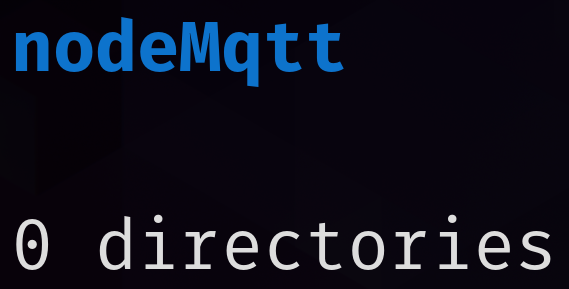
\includegraphics[width=0.7\textwidth]{img/diagramas/directorios_nodeMqtt.png}
%\caption{No tiene rama de directorios de nodeMqtt.}
%\end{figure}

\begin{table}[htbp]
\begin{center}
\caption{Directorio: nodeMqtt.}
\begin{tabular}{|l|l|} %|c|c|
\hline
\rowcolor[HTML]{C0C0C0} 
\textbf{Nombre de Archivo} & \textbf{Descripción}\\ \hline
index.js & Archivo javascript principal\\ \hline
package.json & Información de dependencias\\ \hline
\end{tabular}
\label{tabla:directorioNodeMqtt}
\end{center}
\end{table}

\subsection{InverIoT}
Es una Aplicación de escritorio para el sismtema operativo Windows.

Fue desarrollada usando el lenguaje de programación C\#, permite ver los datos en tiempo real, el histórico de datos y activar mecanismos (representado por la activación de un led verde).

La obtención de datos en tiempo real y las órdenes para activar mecanismos se hace por medio de MQTT~\cite{manual:MQTT}.

La obtención del histórico de datos se hace por medio del protocolo Mysql.

\begin{figure}[h]
\centering

\includegraphics[width=0.7\textwidth]{img/diagramas/directorios_InverIoT.png}
\caption{Rama de directorios de InverIoT.}
\end{figure}

\begin{table}[htbp]
\begin{center}
	\caption{Directorio: InverIoT.}
\begin{tabular}{|l|} %|c|c|
\hline
\rowcolor[HTML]{C0C0C0} 
\textbf{Nombre de Archivo}\\ \hline
favicon.ico \\ \hline
frmGraficas.cs \\ \hline
frmGraficas.Designer.cs \\ \hline
frmGraficas.resx  \\ \hline
frmHistorico.cs  \\ \hline
frmHistorico.Designer.cs  \\ \hline
frmHistorico.resx  \\ \hline
frmMain.cs  \\ \hline
frmMain.Designer.cs  \\ \hline
frmMain.es-ES.resx  \\ \hline
frmMain.resx  \\ \hline
Funciones.cs  \\ \hline
img  \\ \hline
'Instalador - InverIoT - v2.2.exe'  \\ \hline
InverIoT.csproj  \\ \hline
InverIoT.sln  \\ \hline
Program.cs  \\ \hline
README.md  \\ \hline
\end{tabular}
\label{tabla:directorioInverIoT}
\end{center}
\end{table}

\subsection{dashboard}
Este dashboard web permite acceder a los datos en tiempo real y también ver el histórico de datos. No envía ordenes, solo recepciona datos mediante MQTT~\cite{manual:MQTT} y Mysql~\cite{misc:Mysql}.

\begin{figure}[h]
\centering
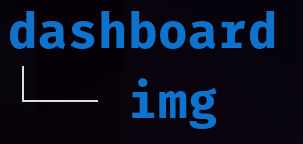
\includegraphics[width=0.7\textwidth]{img/diagramas/directorios_dashboard.png}
\caption{Rama de directorios de dashboard.}
\end{figure}

\begin{table}[htbp]
\begin{center}
\caption{Directorio: dashboard.}
\begin{tabular}{|l|l|} %|c|c|
\hline
\rowcolor[HTML]{C0C0C0} 
\textbf{Nombre de Archivo} & \textbf{Descripción}\\ \hline
android-chrome-192x192.png & Ícono\\ \hline
android-chrome-512x512.png & Ícono\\ \hline
apple-touch-icon.png & Ícono\\ \hline
favicon-16x16.png & Ícono\\ \hline
favicon-32x32.png & Ícono\\ \hline
favicon.ico & Ícono\\ \hline
historico.html & Estructura visual del historial\\ \hline
img & Imágenes del dashboard funcionando\\ \hline
index.html & Estructura visual por defecto\\ \hline
package.json & Dependencias y configuraciones\\ \hline
servers.js & Hace funcionar el dashboard\\ \hline
site.webmanifest & Manifiesto web\\ \hline
\end{tabular}
\label{tabla:directorioDashboard}
\end{center}
\end{table}


\subsection{AnalisisDatos}
Limpia los datos y da un resumen estadístico usando Jupyter Notebook~\cite{misc:Jupyter_Notebook} y el lenguaje de programación Python.

El archivo \textbf{analisis.ipynb} contiene todo el código de programación utilizado en el proceso. 

El archivo \textbf{data.csv} es solo una muestra representativa de los datos, los cuales siguen creciendo conforme siga en funcionamiento el sistema.

La librería de python que principalmente fue usada es \textbf{pandas}.

La recopilación de datos abrirá otras posibilidades de investigación para futuros análisis usando herramientas como machine learning. Por ahora solo nos centramos en almacenar los datos y ver las anomalías que puedan surgir antes de hacer un análisis, es decir, respecto a la limpieza de datos.

%\begin{figure}[h]
%\centering
%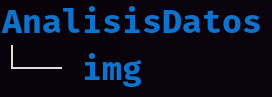
\includegraphics[width=1\textwidth]{img/diagramas/directorios_AnalisisDatos.png}
%\caption{Rama de directorios de AnalisisDatos.}
%\end{figure}

\begin{table}[htbp]
\begin{center}
\caption{Directorio: AnalisisDatos.}
\begin{tabular}{|l|l|} %|c|c|
\hline
\rowcolor[HTML]{C0C0C0} 
\textbf{Nombre de Archivo} & \textbf{Descripción}\\ \hline
analisis.ipynb & Jupyter notebook para analizar datos\\ \hline
data.csv & Data de los sensores\\ \hline
img & Directorio de imágenes \\ \hline
\end{tabular}
\label{tabla:directorioAnalisisDatos}
\end{center}
\end{table}


\subsection{TFG}
Documentación del proyecto usando \LaTeX.

Los archivos principales son \textbf{memoria.tex} y \textbf{anexos.tex} como se puede ver en la tabla~\ref{tabla:TFG}.

\begin{figure}[h]
\centering
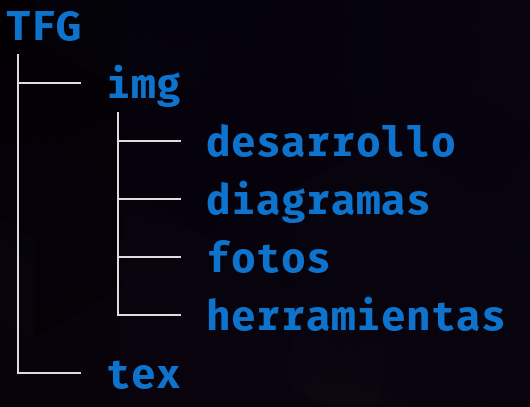
\includegraphics[width=0.7\textwidth]{img/diagramas/directorios_TFG.png}
\caption{descripcion}
\end{figure}

\begin{table}[htbp]
\begin{center}
\caption{Directorio: TFG.}
\begin{tabular}{|l|l|} %|c|c|
\hline
\rowcolor[HTML]{C0C0C0} 
\textbf{Nombre de Archivo} & \textbf{Descripción}\\ \hline
anexos.pdf & PDF de  anexos\\ \hline
anexos.tex & documentación técnica\\ \hline
bibliografiaAnexos.bib & Referencia bibliográficas de anexos.tex\\ \hline
bibliografia.bib & Referencia bibliográficas de memoria.tex\\ \hline
img & directorio de imágenes \\ \hline
memoria.pdf & Resultado de memoria.tex\\ \hline
memoria.tex & Descripción de conceptos y del proyecot en sí\\ \hline
tex & Archivos usados por memoria.tex y anexos.tex\\ \hline
\end{tabular}
\label{tabla:TFG}
\end{center}
\end{table}

\begin{table}[htbp]
\begin{center}
\caption{Directorio: img.}
\begin{tabular}{|l|l|}
\hline
\rowcolor[HTML]{C0C0C0} 
\textbf{Nombre de Archivo} & \textbf{Descripción}\\ \hline
cabecera.pdf & Cabecera con el nombre de la universidad\\ \hline
desarrollo & Imágenes que representan el proceso\\ \hline
diagramas & Esquemas del hardware y diagramas\\ \hline
escudoInfor.pdf & Escudo de la universidad\\ \hline
fotos & Fotos relacionadas al proyecto\\ \hline
herramientas & Imágenes de herramientas usadas\\ \hline
\end{tabular}
\end{center}
\end{table}

\begin{table}[htbp]
\begin{center}
\caption{Directorio: tex.}
\begin{tabular}{|l|}
\hline
\rowcolor[HTML]{C0C0C0} 
\textbf{Nombre de Archivo} \\ \hline
1\_Introduccion.tex \\ \hline
2\_Objetivos\_del\_proyecto.tex \\ \hline
3\_Conceptos\_teoricos.tex \\ \hline
4\_Tecnicas\_y\_herramientas.tex \\ \hline
5\_Aspectos\_relevantes\_del\_desarrollo\_del\_proyecto.tex \\ \hline
6\_Trabajos\_relacionados.tex \\ \hline
7\_Conclusiones\_Lineas\_de\_trabajo\_futuras.tex \\ \hline
A\_Plan\_proyecto.tex \\ \hline
B\_Requisitos.tex \\ \hline
C\_Diseno.tex \\ \hline
D\_Manual\_programador.tex \\ \hline
E\_Manual\_usuario.tex \\ \hline
F\_ODS.tex \\ \hline
\end{tabular}
\end{center}
\end{table}

\section{Manual del programador}
Este apartado describe los recursos y las estrategias para el desarrollo del código, incluyendo una explicación detallada de las diferentes partes del proyecto.

Veremos las instalaciones y configuraciones necesarias para todo funcione correctamente, tanto referente a software y hardware.

El usuario final no tiene porque hacer todas estas configuraciones, él solo tendrá que ejecutar ciertas cosas específicas y muy puntuales.

Se va explicar respecto a las partes que conforman la totalidad de este proyecto:

\begin{table}[htbp]
\begin{center}
\caption{Directorio: Totalidad del proyecto.}
\begin{tabular}{|l|l|}
\hline
\rowcolor[HTML]{C0C0C0} 
\textbf{Parte del proyecto} & \textbf{Descripción}\\ \hline
Servidor LAMP & Gestiona la base de datos y MQTT\\ \hline
Hardware &  Implementación del harware\\ \hline
nodeMqtt & Servicio para almacenar datos en una base de datos \\ \hline
InverIoT &  Aplicación de escritorio\\ \hline
dashboard &  Dashboard web accesible desde internet \\ \hline
AnalisisDatos & Limpieza de datos y resumen estadístico \\ \hline
Bot de Telegram & Recibe alertas y envía comandos \\ \hline
\end{tabular}
\label{tabla:totalidadProyectoFuncional}
\end{center}
\end{table}

\subsection{Servidor LAMP}
Se está usando un servidor físico HP Proliant~\cite{misc:HP_ProLiant}, mediante Hyper-V se ha virtualizado el sistema operativo Ubuntu para el servidor. Se ha hecho esto porque el servidor físico tiene como sistema operativo principal a Windows Server.

El servidor LAMP consta principalmente de un sistema operativo Linux, que en este caso es Ubuntu~\cite{misc:Ubuntu}, Apache~\cite{misc:Apache}, Mysql~\cite{misc:Mysql} y PHP.

Adicionalmente se instalaron otros servicios que se vieron necesarios. La instalación en Ubuntu se hace mediante comandos en la terminal. La descripción de servicio instalado se menciona en la tabla~\ref{tabla:serviciosLAMP}.

\begin{table}[htbp]
\begin{center}
\caption{Características del servidor HP ProLiant.}
\begin{tabular}{|l|l|}
\hline
\rowcolor[HTML]{C0C0C0} 
\textbf{Característica} & \textbf{Descripción}\\ \hline
Sistema operativo & Windows Server 2019 Standard\\ \hline
Fabricante & Hewlett Packard Enterprise \\ \hline
Modelo & Hewlett Packard Enterprise x64 Class PC\\ \hline
Procesador & Intel(R) Xeon(R) Silver 4210R CPU @ 2.4GHz 2.39GHz\\ \hline
Memoria instalada (RAM) & 128 GB (128 GB utilizable) \\ \hline
Tipo de sistema & Sistema operativo de 64 bits, procesador x64 \\ \hline
\end{tabular}
\end{center}
\end{table}

\begin{lstlisting}[language=sh, firstnumber=0, basicstyle=\normalsize, caption={Comando para instalar apache2 .}] 
sudo apt install apache2 \end{lstlisting}

\begin{lstlisting}[language=sh, firstnumber=0, basicstyle=\normalsize, caption={Comando para instalar Mysql.}] 
sudo apt install mysql-server \end{lstlisting}

\begin{lstlisting}[language=sh, firstnumber=0, basicstyle=\normalsize, caption={Comando para instalar PHP.}] 
sudo apt install php \end{lstlisting}

\begin{lstlisting}[language=sh, firstnumber=0, basicstyle=\normalsize, caption={Comando para instalar ssh.}] 
sudo apt install ssh \end{lstlisting}

\begin{lstlisting}[language=sh, firstnumber=0, basicstyle=\normalsize, caption={Comando para instalar phpmyadmin.}] 
sudo apt install phpmyadmin \end{lstlisting}

\begin{lstlisting}[language=sh, firstnumber=0, basicstyle=\normalsize, caption={Comando para instalar vsftpd.}] 
sudo apt install vsftpd\end{lstlisting}

\begin{lstlisting}[language=sh, firstnumber=0, basicstyle=\normalsize, caption={Comando para instalar ufw.}] 
sudo apt install ufw\end{lstlisting}


\begin{lstlisting}[language=sh, firstnumber=0, basicstyle=\normalsize, caption={Comando para instalar node.js.}] 
sudo apt install nodejs\end{lstlisting}

\begin{lstlisting}[language=sh, firstnumber=0, basicstyle=\normalsize, caption={Comando para instalar pm2.}] 
sudo apt install pm2\end{lstlisting}

\begin{lstlisting}[language=sh, firstnumber=0, basicstyle=\normalsize, caption={Comando para instalar mosquitto.}] 
sudo apt install mosquitto\end{lstlisting}

\begin{lstlisting}[language=sh, firstnumber=0, basicstyle=\normalsize, caption={Comando para instalar npm.}] 
sudo apt install npm\end{lstlisting}

\begin{lstlisting}[language=sh, firstnumber=0, basicstyle=\normalsize, caption={Comando para instalar express.}] 
sudo apt install express\end{lstlisting}

Ahora usando mysql crearemos la base de datos y tablas correspondientes.

\begin{table}[htbp]
\begin{center}
\caption{Base de datos TFG\_UBU.}
\begin{tabular}{|l|l|} %|c|c|
\hline
\rowcolor[HTML]{C0C0C0} 
\textbf{Nombre de tabla} & \textbf{Descripción}\\ \hline
sensores &  Captura la fecha, hora y valores de sensores\\ \hline
umbrales & Captura los umbrales \\ \hline
\end{tabular}
\label{tabla:BDTFG}
\end{center}
\end{table}


\begin{lstlisting}[language=sh, firstnumber=0, basicstyle=\normalsize, caption={Comando para acceder a Mysql.}] 
sudo mysql\end{lstlisting}

\begin{lstlisting}[language=python, firstnumber=0, basicstyle=\normalsize, caption={Comandos Mysql para crear Database \textbf{TFG\_UBU}.}] 
CREATE DATABASE TFG_UBU;
CREATE USER 'joseluis'@'%' IDENTIFIED BY 'Mipassword';
GRANT ALL ON TFG_UBU.* TO 'joseluis'@'%';
use TFG_UBU;
\end{lstlisting}


\begin{lstlisting}[language=python, firstnumber=0, basicstyle=\normalsize, caption={Comandos Mysql para crear tabla \textbf{umbrales}.}] 
CREATE TABLE `umbrales` (
  `temperatura_minima` float NOT NULL,
  `temperatura_maxima` float NOT NULL,
  `humedad_ambiente_minima` float NOT NULL,
  `humedad_ambiente_maxima` float NOT NULL,
  `luminosidad_minima` float NOT NULL,
  `luminosidad_maxima` float NOT NULL,
  `humedad_suelo_minima` float NOT NULL,
  `humedad_suelo_maxima` float NOT NULL,
  `fecha_actualizacion` timestamp 
  NULL DEFAULT CURRENT_TIMESTAMP 
  ON UPDATE CURRENT_TIMESTAMP
) ENGINE=InnoDB DEFAULT CHARSET=utf8mb4;
INSERT INTO `umbrales` (
`temperatura_minima`, `temperatura_maxima`, 
`humedad_ambiente_minima`, `humedad_ambiente_maxima`, 
`luminosidad_minima`, `luminosidad_maxima`, 
`humedad_suelo_minima`, `humedad_suelo_maxima`) VALUES
(30, 35, 30, 70, 30, 150, 20, 80);
\end{lstlisting}

\begin{lstlisting}[language=python, firstnumber=0, basicstyle=\normalsize, caption={Comandos Mysql para crear tabla \textbf{sensores}.}] 
CREATE TABLE `sensores` (
  `id` int NOT NULL AUTO_INCREMENT,
  `fecha` date DEFAULT NULL,
  `hora` time DEFAULT NULL,
  `temperatura` decimal(4,2) DEFAULT NULL,
  `humedad` decimal(4,2) DEFAULT NULL,
  `intensidad_luz` decimal(4,2) DEFAULT NULL,
  `humedad_suelo` decimal(4,2) DEFAULT NULL,
  PRIMARY KEY (`id`)
) ENGINE=InnoDB DEFAULT CHARSET=utf8mb4;
\end{lstlisting}

Teniendo en cuenta una configuración de red interna específica, se tiene que reaperturar y redirigir los puertos desde el router para tener acceso al servidor desde el exterior (ip pública), ya que como existen otros servidores sirviendo alguno de los mismos datos, necesitamos redirigir el servicio por puerto.

\begin{table}[htbp]
\begin{center}
\caption{Configuración de red interna.}
\begin{tabular}{|l|l|} %|c|c|
\hline
\rowcolor[HTML]{C0C0C0} 
\textbf{Característica} & \textbf{Valor}\\ \hline
inet & 192.0.0.6 \\ \hline
netmask & 255.255.255.0\\ \hline
broadcast & 192.0.0.255 \\ \hline
\end{tabular}
\end{center}
\end{table}

\begin{lstlisting}[language=cpp, firstnumber=0, basicstyle=\normalsize, caption={Comandos para reaperturar y redirigir puertos.}] 
nat server protocol tcp global interface LoopBack 0 3001 inside 192.0.0.6 ftp
nat server protocol tcp global interface LoopBack 0 3002 inside 192.0.0.6 22
nat server protocol udp global interface LoopBack 0 3002 inside 192.0.0.6 22
nat server protocol tcp global interface LoopBack 0 3003 inside 192.0.0.6 www
nat server protocol udp global interface LoopBack 0 3003 inside 192.0.0.6 80
nat server protocol udp global interface LoopBack 0 3001 inside 192.0.0.6 21
nat server protocol tcp global interface LoopBack 0 8080 inside 192.0.0.6 8080
nat server protocol udp global interface LoopBack 0 8080 inside 192.0.0.6 8080
nat server protocol tcp global interface LoopBack 0 135 inside 192.0.0.6 135
nat server protocol udp global interface LoopBack 0 135 inside 192.0.0.6 135
nat server protocol tcp global interface LoopBack 0 3307 inside 192.0.0.6 3307
nat server protocol udp global interface LoopBack 0 3307 inside 192.0.0.6 3307
nat server protocol tcp global interface LoopBack 0 1883 inside 192.0.0.6 1883
nat server protocol udp global interface LoopBack 0 1883 inside 192.0.0.6 1883
nat server protocol udp global interface LoopBack 0 3000 inside 192.0.0.6 3000
nat server protocol tcp global interface LoopBack 0 3000 inside 192.0.0.6 3000
nat server protocol tcp global interface LoopBack 0 30308 inside 192.0.0.6 3308
nat server protocol udp global interface LoopBack 0 30308 inside 192.0.0.6 3308
\end{lstlisting}

\begin{lstlisting}[language=cpp, firstnumber=0, basicstyle=\normalsize, caption={Comando para activar el firewall.}] 
sudo ufw enable\end{lstlisting}

\begin{lstlisting}[language=cpp, firstnumber=0, basicstyle=\normalsize, caption={Comando para permitir conexión ssh.}] 
sudo ufw allow ssh\end{lstlisting}

\begin{figure}[h]
\centering
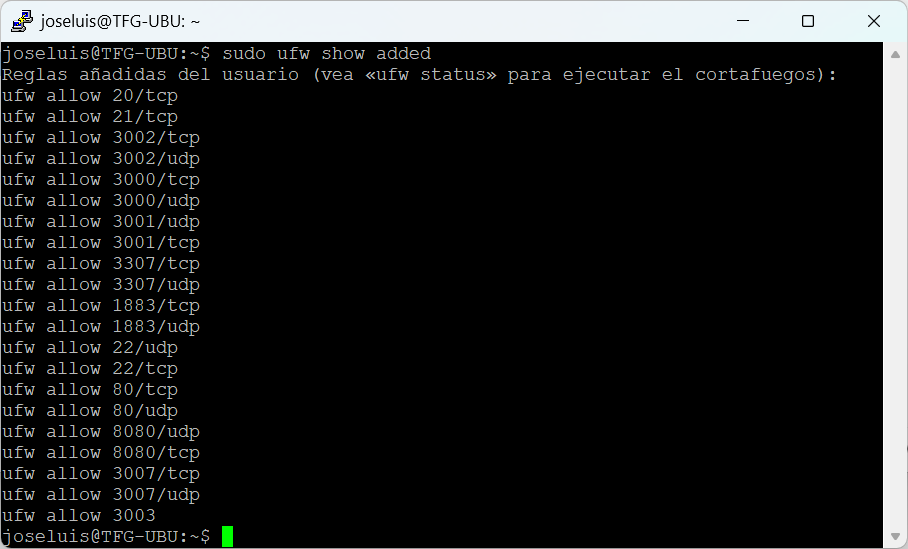
\includegraphics[width=0.5\textwidth]{img/desarrollo/ufw_ShowAdded.png}
\caption{Conexión ssh permitida.}
\end{figure}

Ahora necesitamos instalar \textbf{mosquitto}~\cite{misc:mosquitto} para la conectividad por MQTT~\cite{manual:MQTT}.

MQTT nos servirá para la transmisión de datos en tiempo real, mediante los topics correspondientes.

El servidor LAMP será el Broker MQTT, se encarga de gestionar las peticiones.

\begin{lstlisting}[language=cpp, firstnumber=0, basicstyle=\normalsize, caption={Comando para instalar mosquitto.}] 
sudo apt install mosquitto\end{lstlisting}

\begin{lstlisting}[language=cpp, firstnumber=0, basicstyle=\normalsize, caption={Comando para instalar mosquitto-clients.}] 
sudo apt install mosquitto-clients\end{lstlisting}

\begin{lstlisting}[language=cpp, firstnumber=0, basicstyle=\normalsize, caption={Comando para instalar mosquitto-clients.}] 
sudo apt install mosquitto-clients\end{lstlisting}

\begin{lstlisting}[language=cpp, firstnumber=0, basicstyle=\normalsize, caption={Comando para comprobar el estado de mosquitto.}] 
sudo systemctl status mosquitto\end{lstlisting}

\begin{figure}[h]
\centering
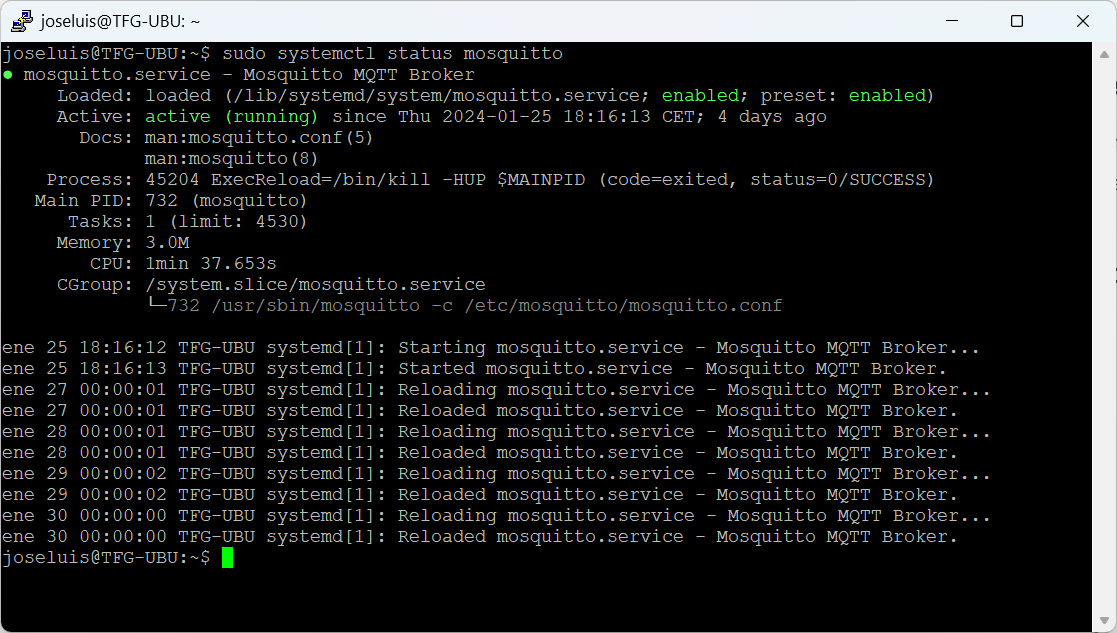
\includegraphics[width=1\textwidth]{img/desarrollo/mosquitto_estado.png}
\caption{Mosquitto operativo}
\end{figure}

\subsection{Hardware}


Se tiene que instalar el firmware en la Raspberry Pi Pico W para que podamos programarlo mediante Micropython.
Primero descargamos el firmware de Micropython desde su página oficial~\cite{misc:MicropythonFirmware}.

Para fines prácticos nombraremos al firmware descargado: \textbf{rp2-pico.uf2}.

\begin{figure}[h]
\centering
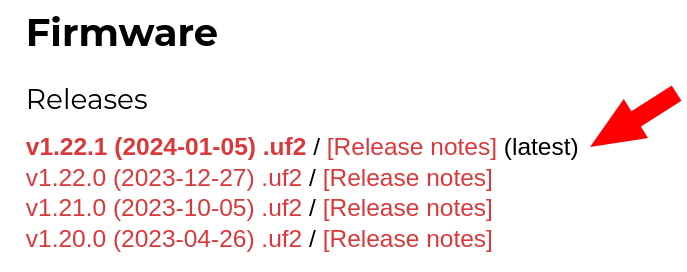
\includegraphics[width=0.7\textwidth]{img/herramientas/micropython_firmware.png}
\caption{Descargar el firmware más reciente.}
\end{figure}

Conectar el puerto usb de la Raspberry Pi Pico W manteniendo presionado el botón \textbf{BOOTSEL}.

\begin{figure}[h]
\centering
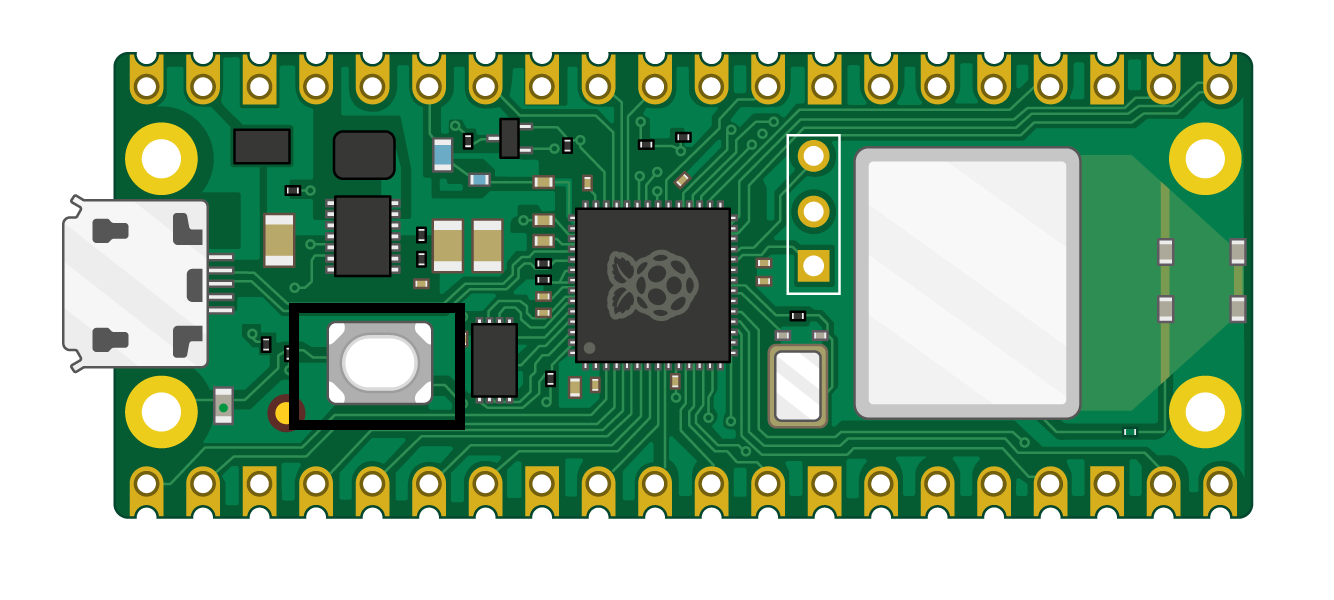
\includegraphics[width=0.7\textwidth]{img/herramientas/rpipicow_boton.png}
\caption{Conectar usb manteniendo presionado.}
\end{figure}

Se ha creado un script en bash al que llamamos \textbf{instaladorFirmware.sh}. La ejecución de este permitirá instalar el firmware de Micropython en la Raspberry Pi Pico W.


\begin{lstlisting}[language=sh, firstnumber=0, basicstyle=\normalsize, caption={Script en bash para instalar el firmware Micropython.}] 
puerto=$(sudo dmesg | tail | grep -o 'sd[b-z]1')
sudo mkdir /mnt/pico
sudo mount /dev/$puerto /mnt/pico
sudo cp rp2-pico.uf2 /mnt/pico
sudo sync
\end{lstlisting}

Tener presente que el archivo \textbf{instaladorFirmware.sh} y el firmware descargado, deben estar en el mismo directorio.

\begin{lstlisting}[language=sh, firstnumber=0, basicstyle=\normalsize, caption={Comando para ejecutar el instalador de Firmware.}] 
sudo ./instaladorFirmware.sh\end{lstlisting}

Ahora que el firmware ya está cargado en la Raspberry Pi Pico W, se le conectan los sensores, módulos y leds RGB tal como se muestra.

\begin{figure}[h]
	\centering
	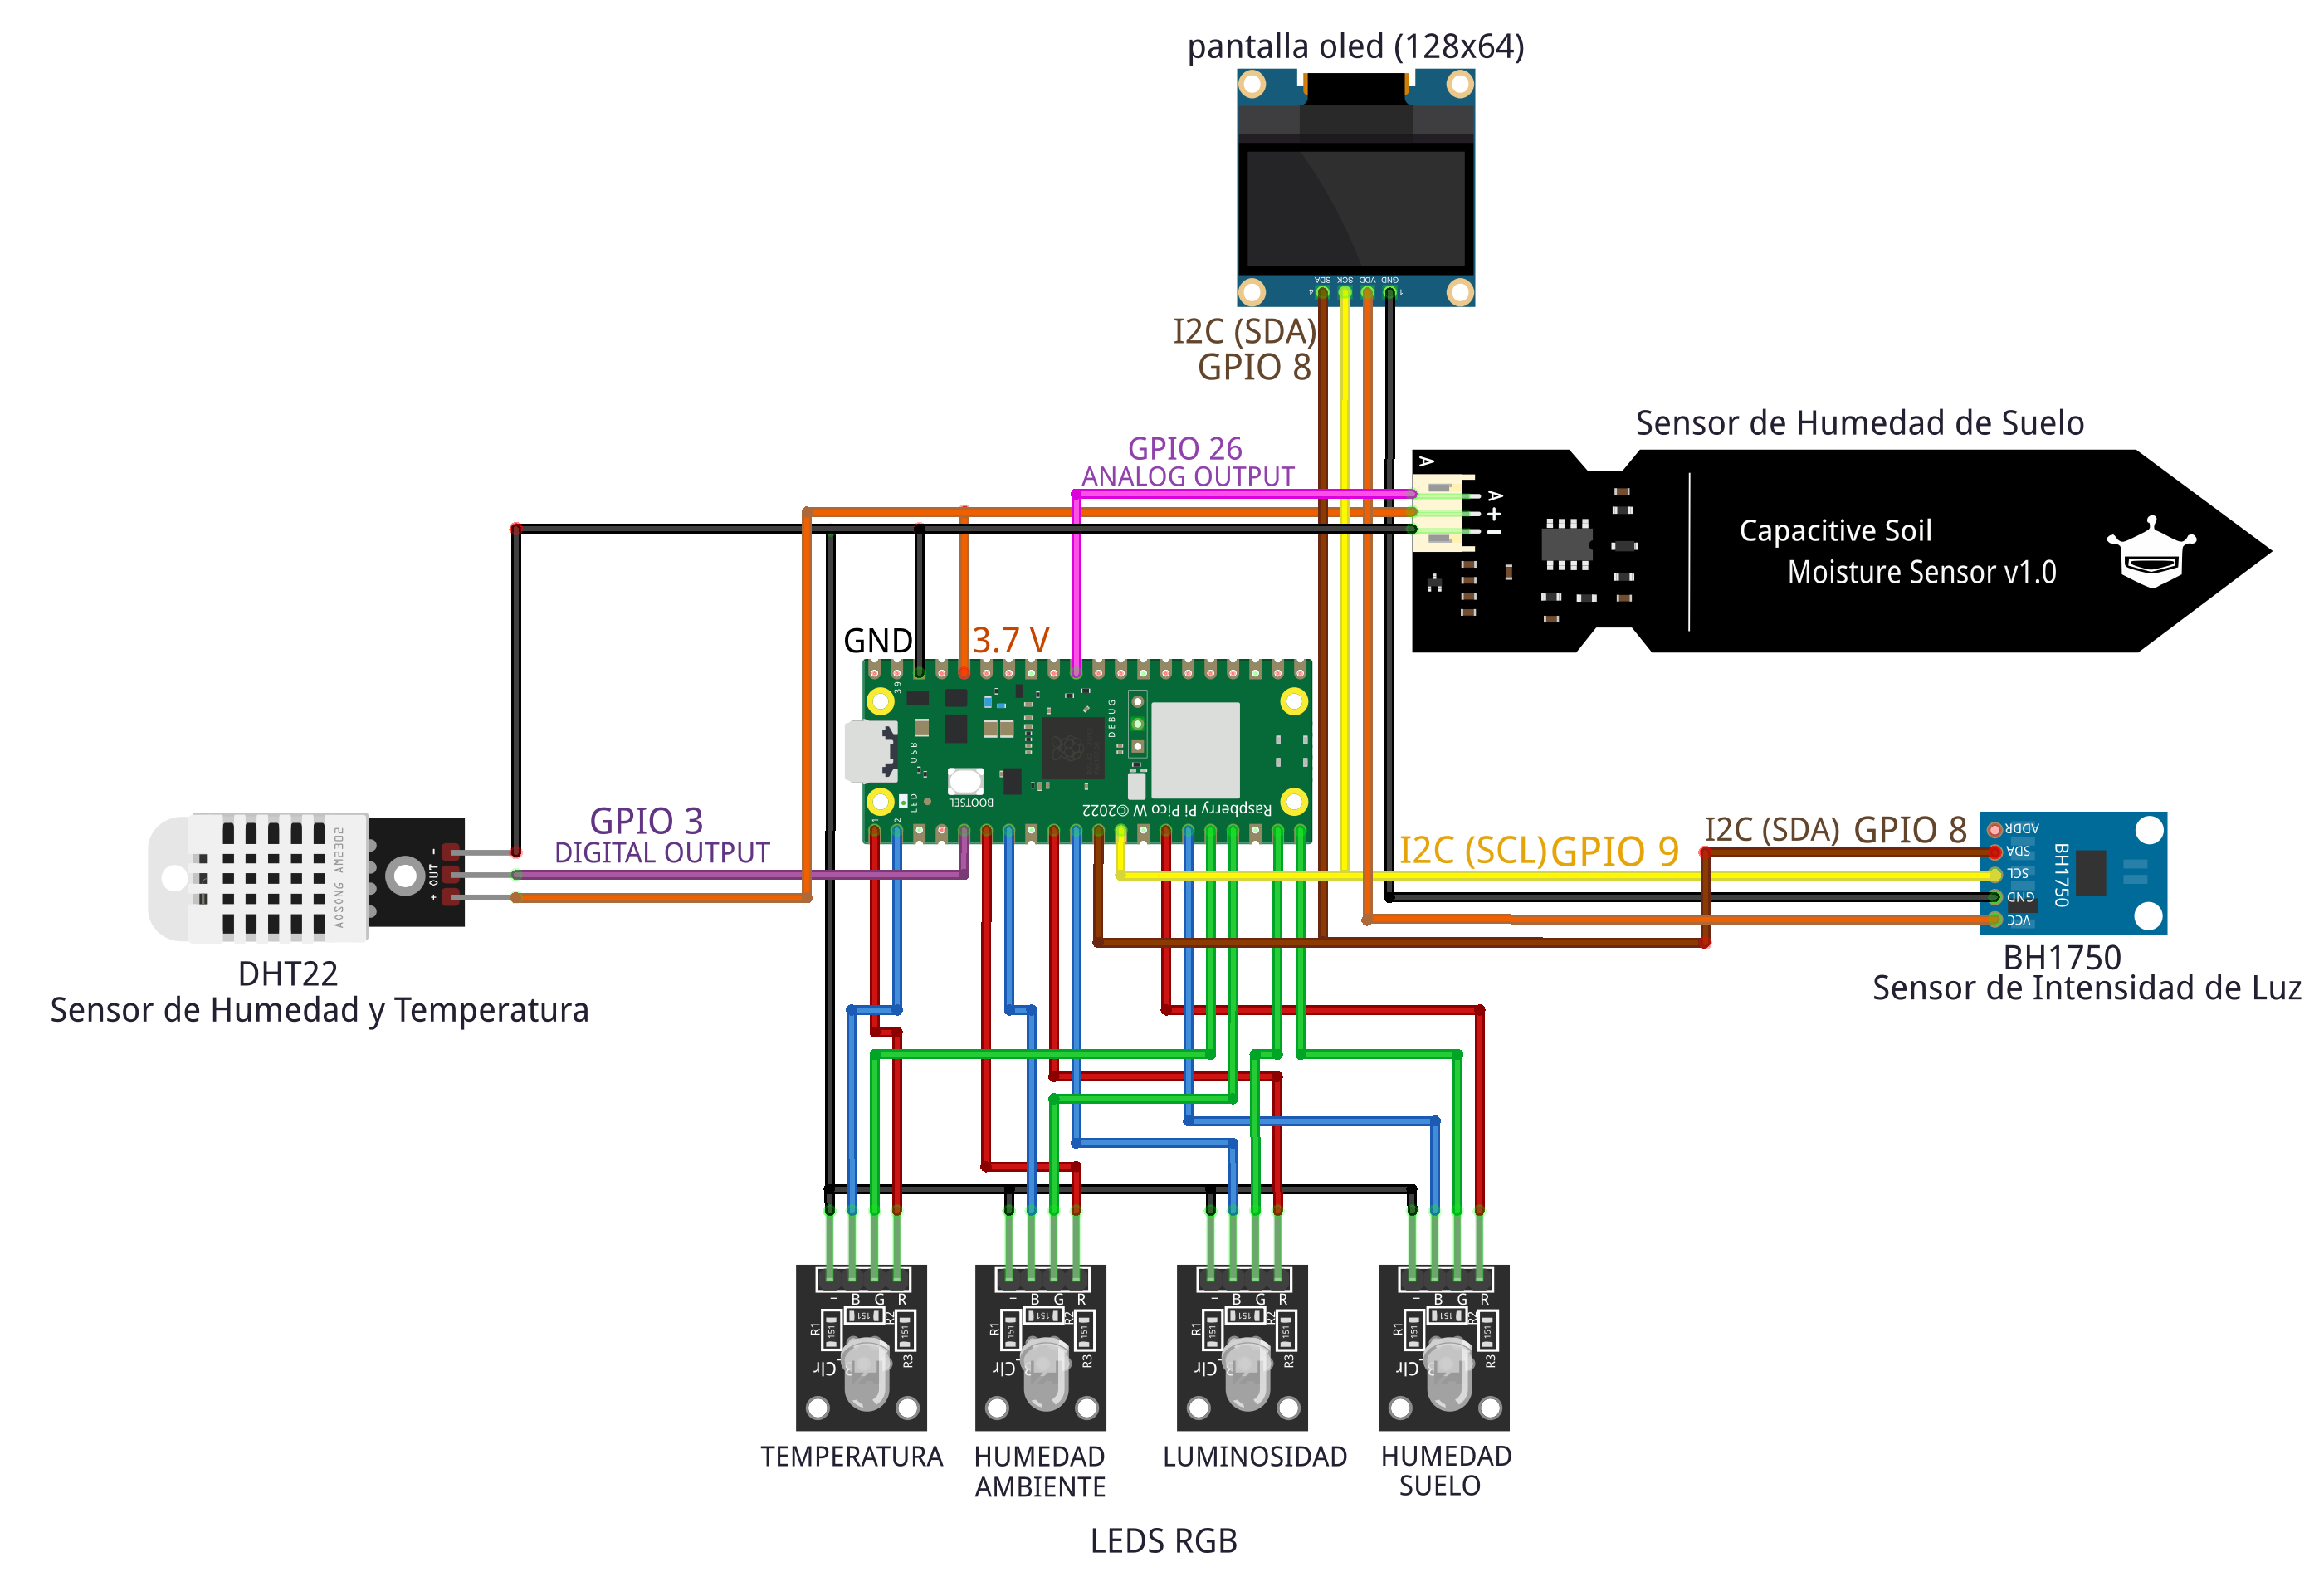
\includegraphics[width=1\textwidth]{img/diagramas/conexiones_simple.png}
	\caption{conexiones en el hardware.}
\end{figure}

Para llevar a cabo estas conexiones, se utiliza un protoboard junto con cables diseñados específicamente para conexiones en este tipo de placas experimentales.

Todos los componentes comparten la misma fuente de alimentación de energía proporcionada por la Raspberry Pi Pico W.

Por ahora ninguno de los componentes necesita alimentación de energía adicional.

Procederemos a mostrar las conexiones específicas de cada componente para más detalle.

\begin{figure}[h]
	\centering
	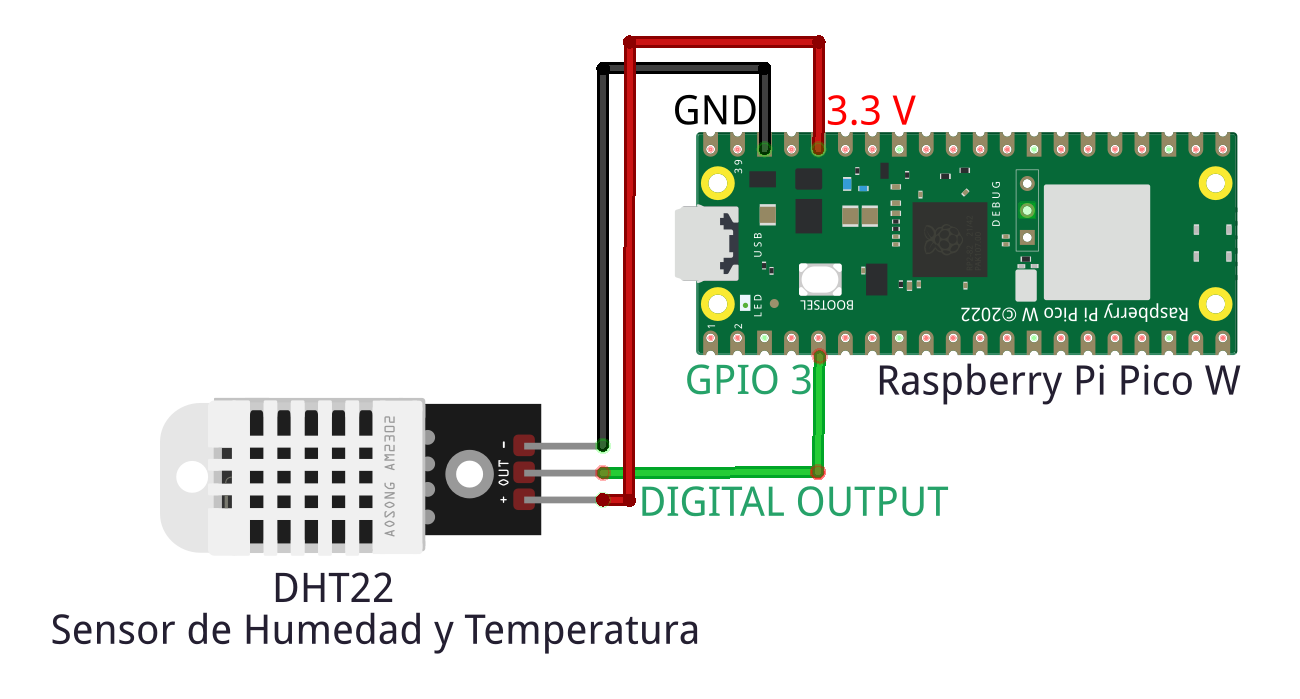
\includegraphics[width=1\textwidth]{img/diagramas/DHT22.png}
	\caption{DHT22: Sensor de humedad y temperatura del ambiente.}
\end{figure}

\begin{figure}[h]
	\centering
	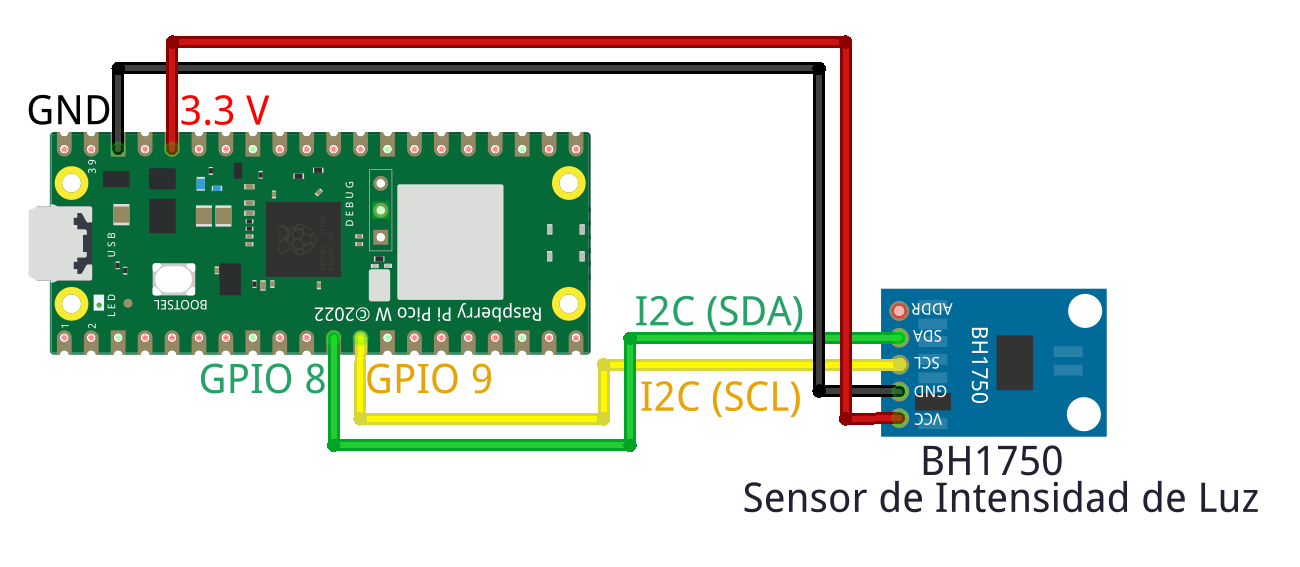
\includegraphics[width=1\textwidth]{img/diagramas/BH1750.png}
	\caption{BH1750: Sensor de intensida de luz.}
\end{figure}

Los diagramas de conexiones son muy claros, no hay gran dificultad para ello.


Respecto a todo el hardware usado, todos los compomentes son de fácil adquisición y hay gran documentación en internet.


\begin{figure}[h]
	\centering
	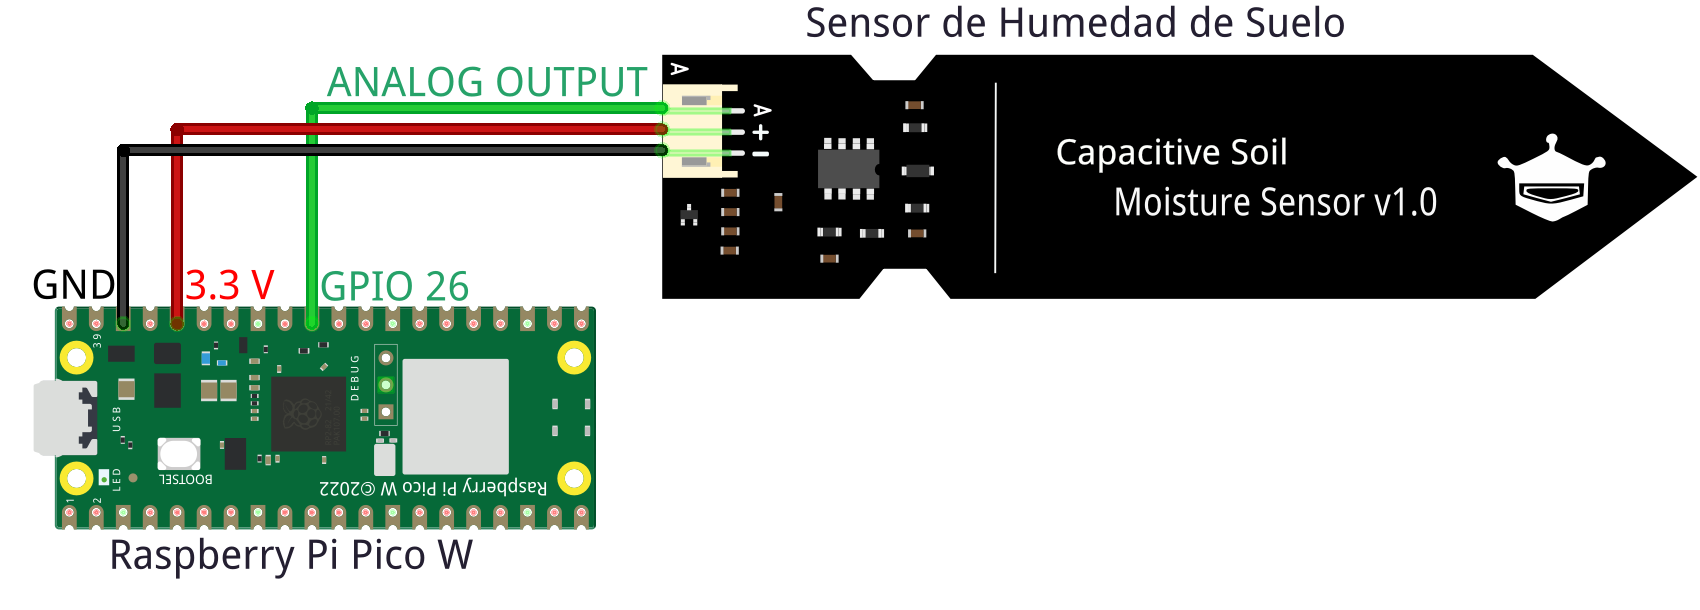
\includegraphics[width=1\textwidth]{img/diagramas/Sensor_humedad_suelo.png}
	\caption{Sensor de humedad del suelo.}
\end{figure}

Si bien por ahora las conexiones se hacen usando un protoboard, en un futuro se puede diseñar una placa para conectar todos los componentes sin necesidad de cables.

El sensor de humedad de suelo~\cite{wiki:SensorHumedadSuelo} debe introducirse en el suelo solo hasta cierto límite.

La pantalla oled~\ref{conexion:oled} permitirá observar los valores de los sensores en tiempo real en el mismo invernadero. Se ha escogido este modelo de pantalla por su bajo consumo de energía y el protocolo I2C nos permite hacer menos conexiones a comparación de este mismo modelo de pantalla pero con protocolo SPI.

\begin{figure}[h]
	\centering
	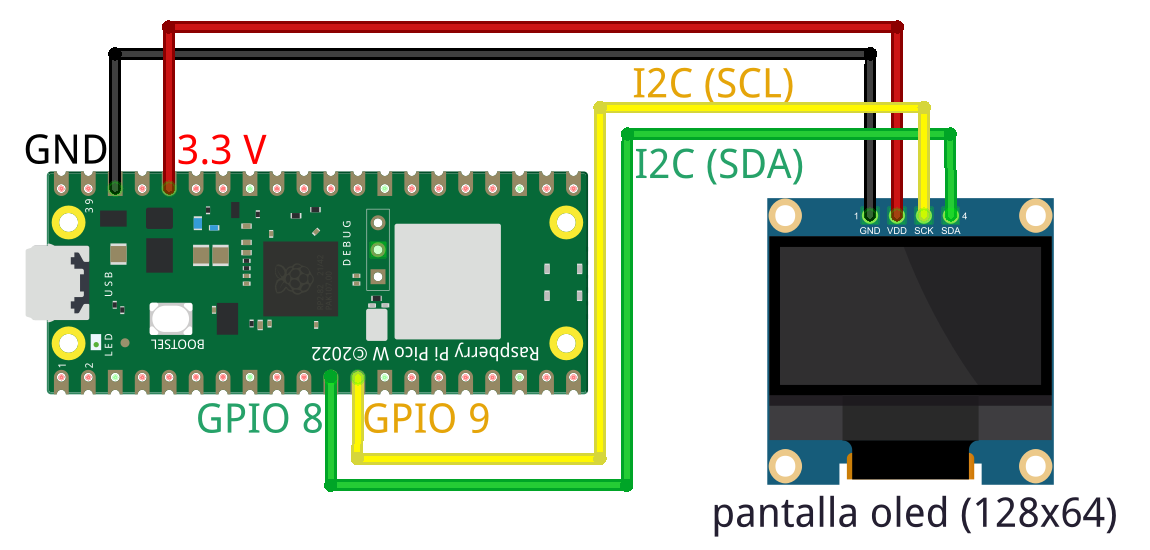
\includegraphics[width=1\textwidth]{img/diagramas/oled.png}
	\caption{Pantalla oled de 128x64 píxeles.}\label{conexion:oled}
\end{figure}

Los leds RGB~\cite{manual:LedRGB} se usarán como alertas visuales, cada color indicará en que posición respecto al umbral está un valor. Los umbrales representan los valores en el que tienen que estar cada una de las variables medidas.

\begin{table}[htbp]
\begin{center}
	\caption{Umbrales ideales para un invernadero de cannabis medicinal.}\label{tabla:umbrales}
\begin{tabular}{|l|l|l|l|}
\hline
\rowcolor[HTML]{C0C0C0} 
\textbf{Característica} & \textbf{Mínimo} & \textbf{Máximo} & \textbf{Unidades}\\ \hline
TEMPERATURA & 30 & 35 & \textcelsius\\ \hline
HUMEDAD & 30 & 70 & \% \\ \hline
LUMINOSIDAD & 30 & 150 & lux\\ \hline
HUMEDAD DEL SUELO & 20 & 80 & \% \\ \hline
\end{tabular}
\label{tabla:umbrales}
\end{center}
\end{table}

\begin{table}[htbp]
\begin{center}
\caption{Indicadores por color en los leds RGB.}
\begin{tabular}{|l|l|} %|c|c|
\hline
\rowcolor[HTML]{C0C0C0} 
\textbf{Color} & \textbf{Descripción}\\ \hline
Rojo & Por encima del umbral\\ \hline
Azul & Por debajo del umbral\\ \hline
Apagado & Valor dentro del umbral\\ \hline
Verde & Mecanismo activado\\ \hline
\end{tabular}
\label{tabla:ledsRGBColores}
\end{center}
\end{table}

Se están usando 4 módulos led RGB, uno por cada variable medida por los sensores.

\begin{figure}[h]
	\centering
	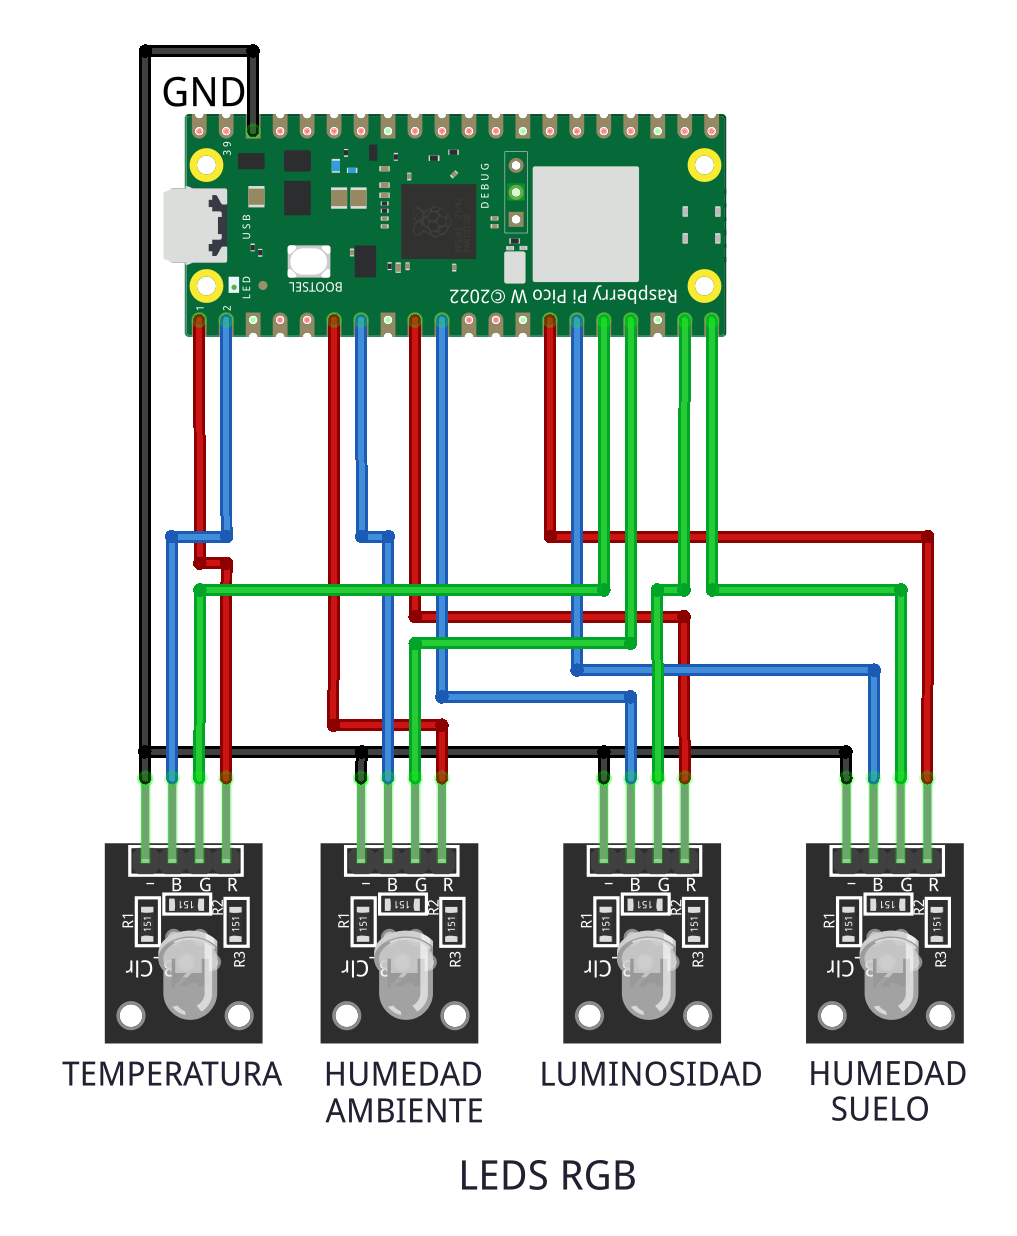
\includegraphics[width=0.5\textwidth]{img/diagramas/leds_rgb.png}
	\caption{Módulo led RGB.}
\end{figure}

Cada módulo RGB tiene un cable para GND y tres respecto a los colores rojo, verde y azul.

Usando el IDE Thonny~\cite{misc:Thonny} y con Micropython vamos a poder programar el hardware. 

Tenemos que hacer unas configuraciones simples antes de poder usar el IDE Thonny con Micropython en nuestra Raspberry Pi Pico W.

Hacemos clic en \textbf{Run/Configure interpreter}.

\begin{figure}[h]
	\centering
	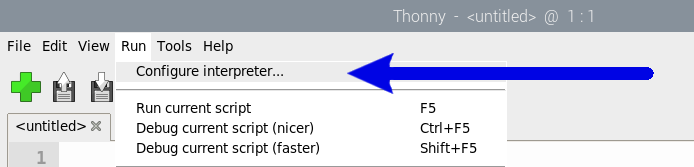
\includegraphics[width=0.8\textwidth]{img/desarrollo/thonny_interpreter.png}
	\caption{Abrimos el configurador del interpreter.}
\end{figure}

Seleccionamos que usaremos \textbf{Micropython} para Raspberry Pi Pico y seleccionamos el puerto que corresponde su conexión por usb.

\begin{figure}[h]
	\centering
	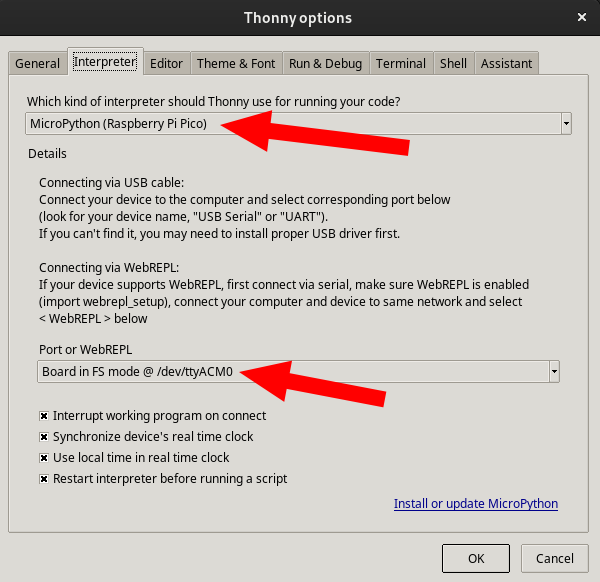
\includegraphics[width=0.8\textwidth]{img/desarrollo/thonny_seleccionInterpreter.png}
	\caption{Habilitamos Thonny para Micropython.}
\end{figure}

Respecto a este proyecto solo tienes que seleccionar el archivo \textbf{main.py} y le das clic en el botón verde para ejecutar y cargar el código a la placa Raspberry Pi Pico W. 

\begin{figure}[h]
	\centering
	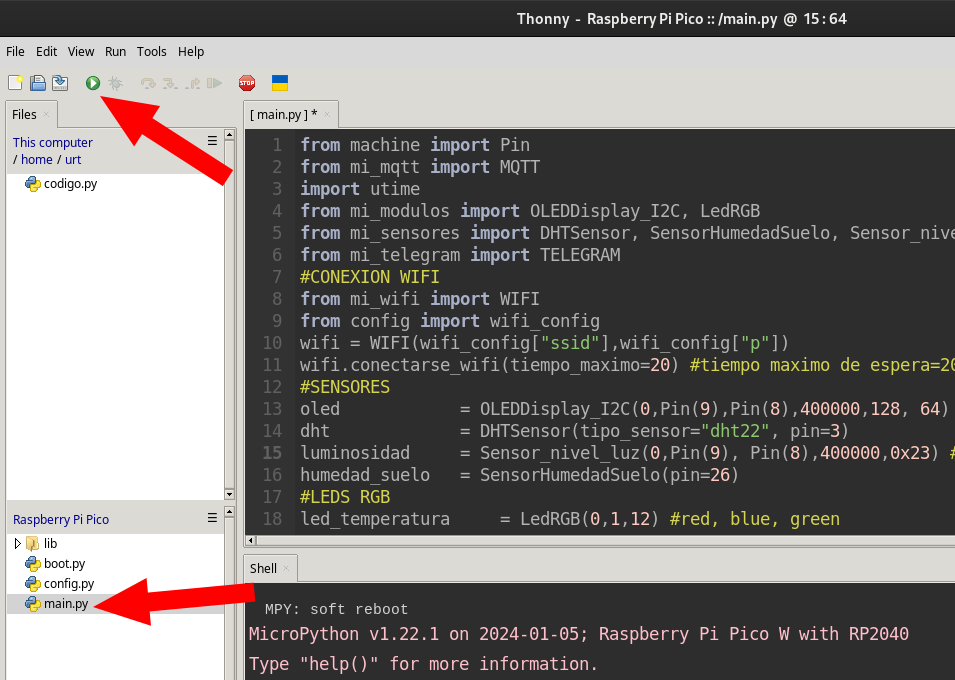
\includegraphics[width=0.65\textwidth]{img/desarrollo/thonny_ejecucion.png}
	\caption{Ejecución y carga a un solo clic.}
\end{figure}

El archivo \textbf{boot.py} se ejecuta al prender la Raspberry Pi Pico W, y al importar el \textbf{main.py} hace que éste se ejecute. Entonces una vez hecha la configuración y programación solo tendremos que suministrar energía a la placa y empezará a funcionar para lo que se le ha programado.

\begin{figure}[h]
	\centering
	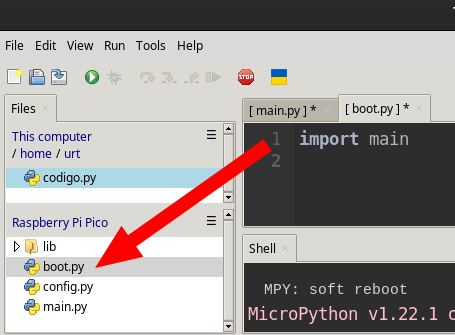
\includegraphics[width=0.65\textwidth]{img/desarrollo/thonny_boot.png}
	\caption{boot.py se ejecuta en el arranque.}
\end{figure}

\subsection{nodeMqtt}

Esta parte del proyecto se encarga de capturar datos mediante MQTT y los almacena en una base de datos usando Mysql. 

La instalación y ejecución es muy simple.

\begin{lstlisting}[language=sh, firstnumber=0, basicstyle=\normalsize, caption={Comando para instalar MQTT.js.}] 
npm install mqtt \end{lstlisting}

\begin{lstlisting}[language=sh, firstnumber=0, basicstyle=\normalsize, caption={Comando para instalar mysql para node.js.}] 
npm install mysql2\end{lstlisting}

\begin{lstlisting}[language=sh, firstnumber=0, basicstyle=\normalsize, caption={Ejecución.}] 
mp2 start index.js --name "nodeMqtt"\end{lstlisting}

Respecto a MQTT \textbf{index.js} utiliza los siguientes topics.

\begin{table}[htbp]
\begin{center}
\caption{Topics MQTT usados en \textbf{nodeMqtt}.}
\begin{tabular}{|l|l|} %|c|c|
\hline
\rowcolor[HTML]{C0C0C0} 
\textbf{Característica} & \textbf{Descripción}\\ \hline
invernadero/sensores &  Captura la fecha, hora y valores de sensores\\ \hline
invernadero/umbrales & Captura los umbrales \\ \hline
\end{tabular}
\end{center}
\end{table}

Almacena los datos en la base de datos \textbf{TFG\_UBU}~\ref{tabla:BDTFG}.

\begin{figure}[h]
	\centering
	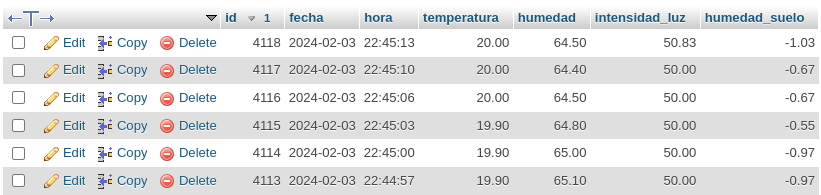
\includegraphics[width=1\textwidth]{img/desarrollo/mysql_tabla_sensores.png}
	\caption{Datos almacenados en tabla.}
\end{figure}

Veamos el contenido de \textbf{index.js}.

\begin{lstlisting}[language=cpp, firstnumber=0, basicstyle=\normalsize, caption={Contenido de index.js.}] 
var mqtt = require("mqtt");
const mysql = require('mysql2');

// Opciones para la conexión MQTT
const mqttOptions = {
  keepAlive: 60,
  reconnectPeriod: 1000,
  connectTimeout: 4000
};

const client = mqtt.connect("mqtt://localhost:1883", mqttOptions);

const dbConfig = {
  host: 'localhost',
  user: 'joseluis',
  password: 'TuPassword',
  database: 'TFG_UBU',
  port: 3307
};
const pool = mysql.createPool(dbConfig);
function EventoConectar() {
  client.subscribe("invernadero/sensores");
  client.subscribe("invernadero/umbrales");
}
function EventoMensaje(topic, message) {
  if (topic === "invernadero/sensores") {
    const [fecha, hora, temperatura, humedad, intensidad_luz, humedad_suelo] = message.toString().split(',');
    const query = 'INSERT INTO sensores (fecha, hora, temperatura, humedad, intensidad_luz, humedad_suelo) VALUES (?, ?, ?, ?, ?, ?)';
    pool.query(query, [fecha, hora, temperatura, humedad, intensidad_luz, humedad_suelo], (error) => {
      if (error) {
        console.error('Error al realizar la inserción en la base de datos:', error);
      } else {
        console.log('Inserción en base de datos exitosa');
      }
    });
  } else if (topic === "invernadero/umbrales") {
    const [temperatura_minima, temperatura_maxima, humedad_minima, humedad_maxima, luminosidad_minima, luminosidad_maxima, humedad_suelo_minima, humedad_suelo_maxima] = message.toString().split(',');

    const query = 'UPDATE umbrales SET temperatura_minima = ?, temperatura_maxima = ?, humedad_ambiente_minima = ?, humedad_ambiente_maxima = ?, luminosidad_minima = ?, luminosidad_maxima = ?, humedad_suelo_minima = ?, humedad_suelo_maxima = ?';

    pool.query(query, [temperatura_minima, temperatura_maxima, humedad_minima, humedad_maxima, luminosidad_minima, luminosidad_maxima, humedad_suelo_minima, humedad_suelo_maxima], (error) => {
      if (error) {
        console.error('Error al actualizar umbrales en la base de datos:', error);
      } else {
        console.log('Actualización de umbrales en base de datos exitosa');
      }
    });
  }
}

client.on("connect", EventoConectar);
client.on("message", EventoMensaje);

pool.on('error', (err) => {
  console.error('Error inesperado en la conexión del pool:', err);
});
\end{lstlisting}

\subsection{InverIoT}
Aplicación de escritorio para Windows usando C\#.

Los archivos relacionados a este proyecto están indicados en la tabla \ref{tabla:directorioInverIoT}.

\begin{table}[htbp]
\begin{center}
\caption{Topics MQTT usados en \textbf{InverIoT}.}
\begin{tabular}{|l|l|}
\hline
\rowcolor[HTML]{C0C0C0} 
\textbf{Característica} & \textbf{Descripción}\\ \hline
invernadero/ordenes & Captura las ordenes\\ \hline
invernadero/sensores &  Captura la fecha, hora y valores de sensores\\ \hline
\end{tabular}
\end{center}
\end{table}

MQTT se usa para mostrar los datos en tiempo real y Mysql para el histórico de datos.

Las ordenes que se envían son para activar mecanismos (representados por la activación de un led verde).

La ejecución del programa lo podemos hacer en Visual Studio Code~\cite{misc:vscode} de la siguiente forma:

\begin{lstlisting}[language=sh, firstnumber=0, basicstyle=\normalsize, caption={Ejecutar proyecto InverIoT.}] 
dotnet build\end{lstlisting}

\begin{lstlisting}[language=cpp, firstnumber=0, basicstyle=\normalsize, caption={Contenido de Program.cs.}] 
namespace InverIoT
{
    internal static class Program
    {
        /// <summary>
        ///  The main entry point for the application.
        /// </summary>
        [STAThread]
        static void Main()
        {
            // see https://aka.ms/applicationconfiguration.
            ApplicationConfiguration.Initialize();
            Application.Run(new frmMain());
        }
    }
}
\end{lstlisting}

\subsection{dashboard}
Dashboard web para mostrar datos, no envía ordenes. Es accesible desde internet.
El contenido del directorio \textbf{dashboard} lo encontramos en la tabla~\ref{tabla:directorioDashboard}.

\begin{table}[htbp]
\begin{center}
\caption{Topics MQTT usados en \textbf{dashboard}.}
\begin{tabular}{|l|l|} %|c|c|
\hline
\rowcolor[HTML]{C0C0C0} 
\textbf{Característica} & \textbf{Descripción}\\ \hline
invernadero/sensores &  Captura la fecha, hora y valores de sensores\\ \hline
\end{tabular}
\end{center}
\end{table}


\begin{lstlisting}[language=sh, firstnumber=0, basicstyle=\normalsize, caption={Instalaciones necesarias.}] 
npm install express
npm install socket.io
\end{lstlisting}

Respecto al archivo \textbf{servers.js} debemos configurar respecto a la base de datos creada en el servidor LAMP:

\begin{lstlisting}[language=cpp, firstnumber=0, basicstyle=\normalsize, caption={Configuración de base de datos.}] 
const dbConfig = {
    host: 'localhost',
    port: 3307, // Puerto especificado aquí
    user: 'joseluis',
    password: 'TuPassword',
    database: 'TFG_UBU'
};
\end{lstlisting}

\begin{lstlisting}[language=sh, firstnumber=0, basicstyle=\normalsize, caption={Ejecución.}] 
mp2 start servers.js --name "dashboard"
\end{lstlisting}

\begin{lstlisting}[language=cpp, firstnumber=0, basicstyle=\normalsize, caption={Contenido de \textbf{servers.js}.}] 
const express = require('express');
const http = require('http');
const socketIo = require('socket.io');
const mqtt = require('mqtt');
const path = require('path');
const mysql = require('mysql2');
const cors = require('cors');
const app = express();
const server = http.createServer(app);
const io = socketIo(server);
const mqttClient = mqtt.connect('mqtt://localhost:1883', {
  keepAlive: 60,            // Enviar un mensaje de ping cada 60 segundos para mantener la conexión
  reconnectPeriod: 1000,    // Intentar reconectar cada 1000 milisegundos (1 segundo) en caso de desconexión
  connectTimeout: 4000      // Tiempo de espera de 4000 milisegundos (4 segundos) para la conexión inicial
});
// Configuración de la base de datos
const dbConfig = {
    host: 'localhost',
    port: 3307, // Puerto especificado aquí
    user: 'joseluis',
    password: 'TuPassword',
    database: 'TFG_UBU'
};

const pool = mysql.createPool(dbConfig);
// Intentar obtener una conexión para probar si la conexión a la base de datos es exitosa
pool.getConnection((err, connection) => {
    if (err) {
        console.error('Error al conectar a la base de datos:', err);
        return;
    }
    console.log('Conectado exitosamente a la base de datos MySQL');
    connection.release(); // No olvides liberar la conexión
});

// Conexión a MQTT y manejo de mensajes
mqttClient.on('connect', () => {
    console.log('Conectado al broker MQTT');
    mqttClient.subscribe('invernadero/sensores');
});

mqttClient.on('message', (topic, message) => {
    console.log(`Mensaje recibido en el topic ${topic}: ${message}`);
    if (topic === 'invernadero/sensores') {
        io.emit('mqtt_data', message.toString());
    }
});

// Middleware
app.use(express.static(path.join(__dirname, './')));
app.use(cors());

// Rutas para servir las páginas
app.get('/', (req, res) => {
    res.sendFile(path.join(__dirname, './', 'index.html'));
});
app.get('/historico', (req, res) => {
    res.sendFile(path.join(__dirname, './', 'historico.html'));
});

// Ruta para obtener datos históricos en un rango de fechas
app.get('/datos-historicos', (req, res) => {
    const { fechaInicio, fechaFin } = req.query;
    let query = "SELECT fecha, hora, temperatura, humedad, intensidad_luz, humedad_suelo FROM sensores";
    let params = [];
    if (fechaInicio && fechaFin) {
        query += " WHERE fecha BETWEEN ? AND ?";
        params.push(fechaInicio, fechaFin);
    }
    pool.query(query, params, (error, results, fields) => {
        if (error) {
            console.error('Error al realizar la consulta a la base de datos:', error);
            res.status(500).send('Error al obtener los datos');
            return;
        }
        res.json(results);
    });
});

app.get('/umbrales', (req, res) => {
    pool.query('SELECT * FROM umbrales ORDER BY fecha_actualizacion DESC LIMIT 1', (error, results, fields) => {
        if (error) {
            console.error('Error al realizar la consulta a la base de datos:', error);
            res.status(500).send('Error al obtener los datos de los umbrales');
            return;
        }
        res.json(results[0]);
    });
});
const PORT = 3000;
server.listen(PORT, () => console.log(`Servidor corriendo en el puerto ${PORT}`));
\end{lstlisting}

\begin{figure}[h]
\centering
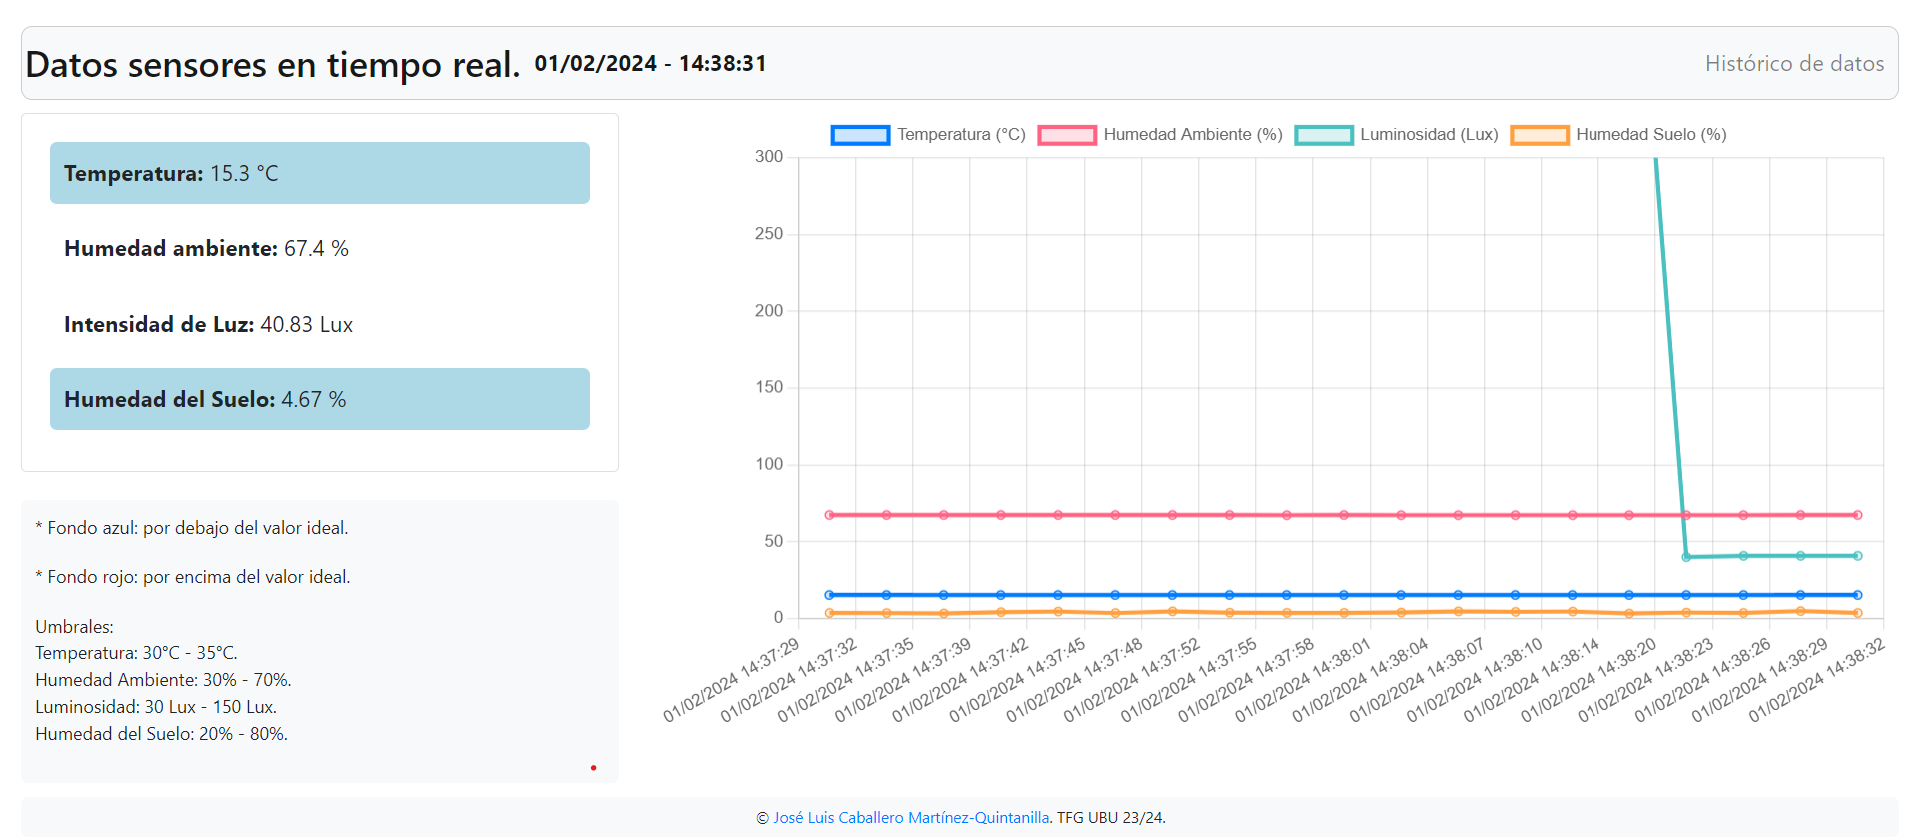
\includegraphics[width=1\textwidth]{img/desarrollo/Dashboard2.png}
\caption{Dashboard en ejecución.}
\end{figure}

\subsection{AnalisisDatos}
Mediante Jupyter Notebook~\cite{misc:Jupyter_Notebook} se hace la limpieza de datos y un resumen estadístico.

En el directorio \textbf{AnalisisDatos}~\ref{tabla:directorioAnalisisDatos} vamos a encontrar los archivos \textbf{analisis.ipynb} y \textbf{data.csv}.

\begin{lstlisting}[language=cpp, firstnumber=0, basicstyle=\normalsize, caption={Instalación de Jupyter Notebook.}] 
sudo apt install jupyter-notebook
\end{lstlisting}

\begin{lstlisting}[language=cpp, firstnumber=0, basicstyle=\normalsize, caption={Ejecución de \textbf{analisis.ipynb}.}] 
jupyter-notebook analisis.ipynb
\end{lstlisting}

Luego automáticamente se ejecuta el notebook y se visualiza en el navegador con una ruta muy similar a esta:

\textbf{http://localhost:8888/notebooks/analisis.ipynb}

Ahora ya puedes ver el código de análisis de datos con python en Jupyter Notebook.

\begin{figure}[h]
\centering
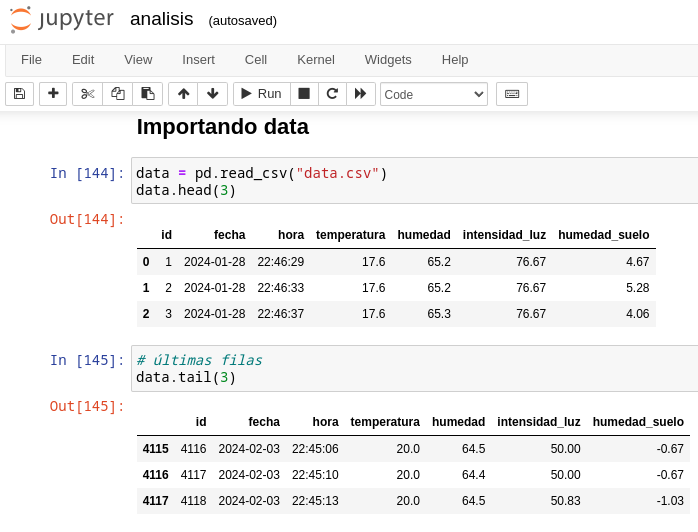
\includegraphics[width=0.9\textwidth]{img/desarrollo/jupyter_inicio.png}
\caption{Data de sensores en Jupyer notebook}
\end{figure}

\section{Compilación, instalación y ejecución del proyecto}
Luego de hacer las configuraciones ya mencionadas, se va a ejecutar respecto a estas partes específicas del proyecto:

\begin{table}[htbp]
\begin{center}
\caption{Compilación y ejecución.}
\begin{tabular}{|l|l|}
\hline
\rowcolor[HTML]{C0C0C0} 
\textbf{Parte del proyecto} & \textbf{Descripción}\\ \hline
Servidor LAMP & Automático\\ \hline
Hardware &  Automático al suministrar energía\\ \hline
nodeMqtt & Automático \\ \hline
InverIoT &  Solo ejecutar su instalador en Windows\\ \hline
dashboard &  Automático \\ \hline
AnalisisDatos & Necesita abrir mediante Jupyter Notebook \\ \hline
Bot de Telegram & Automático \\ \hline
\end{tabular}
\label{tabla:CompilacionEjecucion}
\end{center}
\end{table}

\subsection{Hardware}
Simplemente conectar la Raspberry Pi Pico a una toma de energía y todo el hardware va a empezar a funcionar, ya que se ha configurado para que el archivo \textbf{main.py} se está ejecutando en el arranque.

\subsection{InverIoT}
Se puede usar simplemente su instalador llamado \textbf{Instalador - InverIoT - v2.2.exe}.

O se puede ejecutar el código fuente usando Visual Studio Code~\cite{misc:vscode}.

\begin{lstlisting}[language=sh, firstnumber=0, basicstyle=\normalsize, caption={Ejecutar proyecto InverIoT.}] 
dotnet build\end{lstlisting}

\subsection{AnalisisDatos}

Se ejecuta usando Jupyter Notebook~\cite{misc:Jupyter_Notebook}.

\begin{lstlisting}[language=cpp, firstnumber=0, basicstyle=\normalsize, caption={Ejecución de \textbf{analisis.ipynb}.}] 
jupyter-notebook analisis.ipynb
\end{lstlisting}

\section{Calidad del código}
Para evaluar la calidad del código, se ha empleado un servicio externo denominado SonarCloud, integrado con GitHub. Este servicio realiza un análisis exhaustivo del código, identificando posibles errores y sugiriendo mejoras para optimizar la calidad del código fuente.

Puedes acceder a las estadísticas de SonarCloud mediante el siguiente enlace:~\url{https://sonarcloud.io/project/overview?id=JLCaballeroMQ_Proyecto_TFG_UBU_23_24}

%\section{Pruebas del sistema}
